\label{sec:intro}

Writing multithreaded programs can be challenging. Not only must
programmers cope with the difficulty of writing concurrent programs
(races, atomicity violations, and deadlocks), they must also make sure
they are efficient and scalable. Key to achieving high performance and
scalability is reducing contention for shared resources. However,
threads can still suffer from \emph{false} sharing when multiple
objects that are not logically shared reside on the same cache
line. When false sharing is frequent enough, the resulting
``ping-ponging'' of cache lines across processors can cause
performance to plummet~\cite{falseshare:effect,falseshare:Analysis}.
False sharing can degrade application performance by as much as an
order of magnitude. Two trends---the prevalence of multicore
architectures and the expected increase in the number of multithreaded
applications in broad use, and increasing cache line sizes---are
likely to make false sharing increasingly common.

Locating false sharing requires tool support. Past false sharing
detection tools operate on binaries, either via
simulation~\cite{falseshare:simulator} or binary
instrumentation~\cite{falseshare:binaryinstrumentation1,falseshare:binaryinstrumentation2,zhao:vee:2011}, and intercept all reads and
writes (leading to slowdowns of up to $200\times$), or
rely on hardware performance monitors and correlate cache
invalidations with function calls~\cite{detect:ptu, detect:intel}

These false sharing detection tools suffer from problems that greatly
limit their usefulness. They generate numerous false positives:
addresses that appear shared but are just reused by the memory
allocator, instances of true sharing, and objects that were falsely
shared so few times that they do not present a performance bottleneck.
They also provide little actionable information for programmers
seeking to resolve false sharing in their programs. Their reports
range from a list of suspicious memory addresses with functions that
accessed them at some point~\cite{detect:ptu,falseshare:simulator} to
a single number representing the overall false sharing rate for the
entire
program~\cite{falseshare:binaryinstrumentation1,falseshare:binaryinstrumentation2,zhao:vee:2011}.

This paper presents two tools designed to help programmers effectively address the
challenges of locating and dealing with false sharing in multithreaded
applications. \sheriffdetect{} finds and reports false sharing
accurately (no false positives) and precisely, indicating the exact
objects responsible for false sharing. When rewriting an application
to resolve false sharing is infeasible (because source is unavailable,
or padding data structures would unacceptably reduce cache utilization
and/or increase memory consumption), \sheriffprotect{} can be used as
a runtime system that eliminates false sharing automatically. Both
tools leverage a common framework we introduce here called \sheriff{}
that enables them to operate efficiently.

Figure~\ref{fig:usecase} presents a sample workflow for
using \sheriffdetect{} and \sheriffprotect{}. A multithreaded program
is first executed with \sheriffdetect{} to uncover any false
sharing. The programmer can then act on \sheriffdetect{}'s reports to
correct false sharing by applying padding or aligning objects to cache
line boundaries. If these fixes resolve the problem, then the modified
program can be used with the standard \pthreads{} library. If the
fixes degrade performance or introduce excessive memory
consumption~\cite{zhao:vee:2011}, or when it is impractical or
impossible to modify the program, then \sheriffprotect{} can be used
as a substitute runtime system to automatically eliminate false
sharing.

\subsection*{Contributions}

This paper makes the following contributions:

\begin{itemize}

\item It presents {\bf \sheriff{}}, a software-only framework that replaces
the standard \pthreads{} library and transforms threads into OS
processes. It exposes an API that enables \emph{per-thread memory
protection} and optional \emph{memory isolation} on a per-page
basis. We believe \sheriff{} is of independent interest since it
enables a range of possible applications, including language support
and enforcement of data sharing, software transactional memory,
thread-level speculation, and race detection~\cite{mammoths}, though
we use \sheriff{} here to build two tools focused on false sharing.

\item It presents {\bf \sheriffdetect{}}, a tool that finds and reports false
sharing with high precision and with no false positives. It only
reports actual false sharing---not true sharing, and not artifacts
from heap object reuse. It uses sampling to rank instances of false sharing by
their potential performance impact. \sheriffdetect{} pinpoints false
sharing locations by indicating offsets and global variables or heap
objects (with allocation sites), making false sharing relatively easy
to locate and correct. \sheriffdetect{} is generally efficient: on average, it
slows down execution time by just 20\%.

\item It presents {\bf \sheriffprotect{}}, a tool that eliminates false sharing
automatically without the need for code modifications or
recompilation. \sheriffprotect{} can dramatically increase performance
in the face of false sharing sharing. To our knowledge, \sheriffprotect{} is
the first false sharing resistant runtime for shared-memory
multithreaded programs.

\end{itemize}

\begin{figure}[!t]
\centering
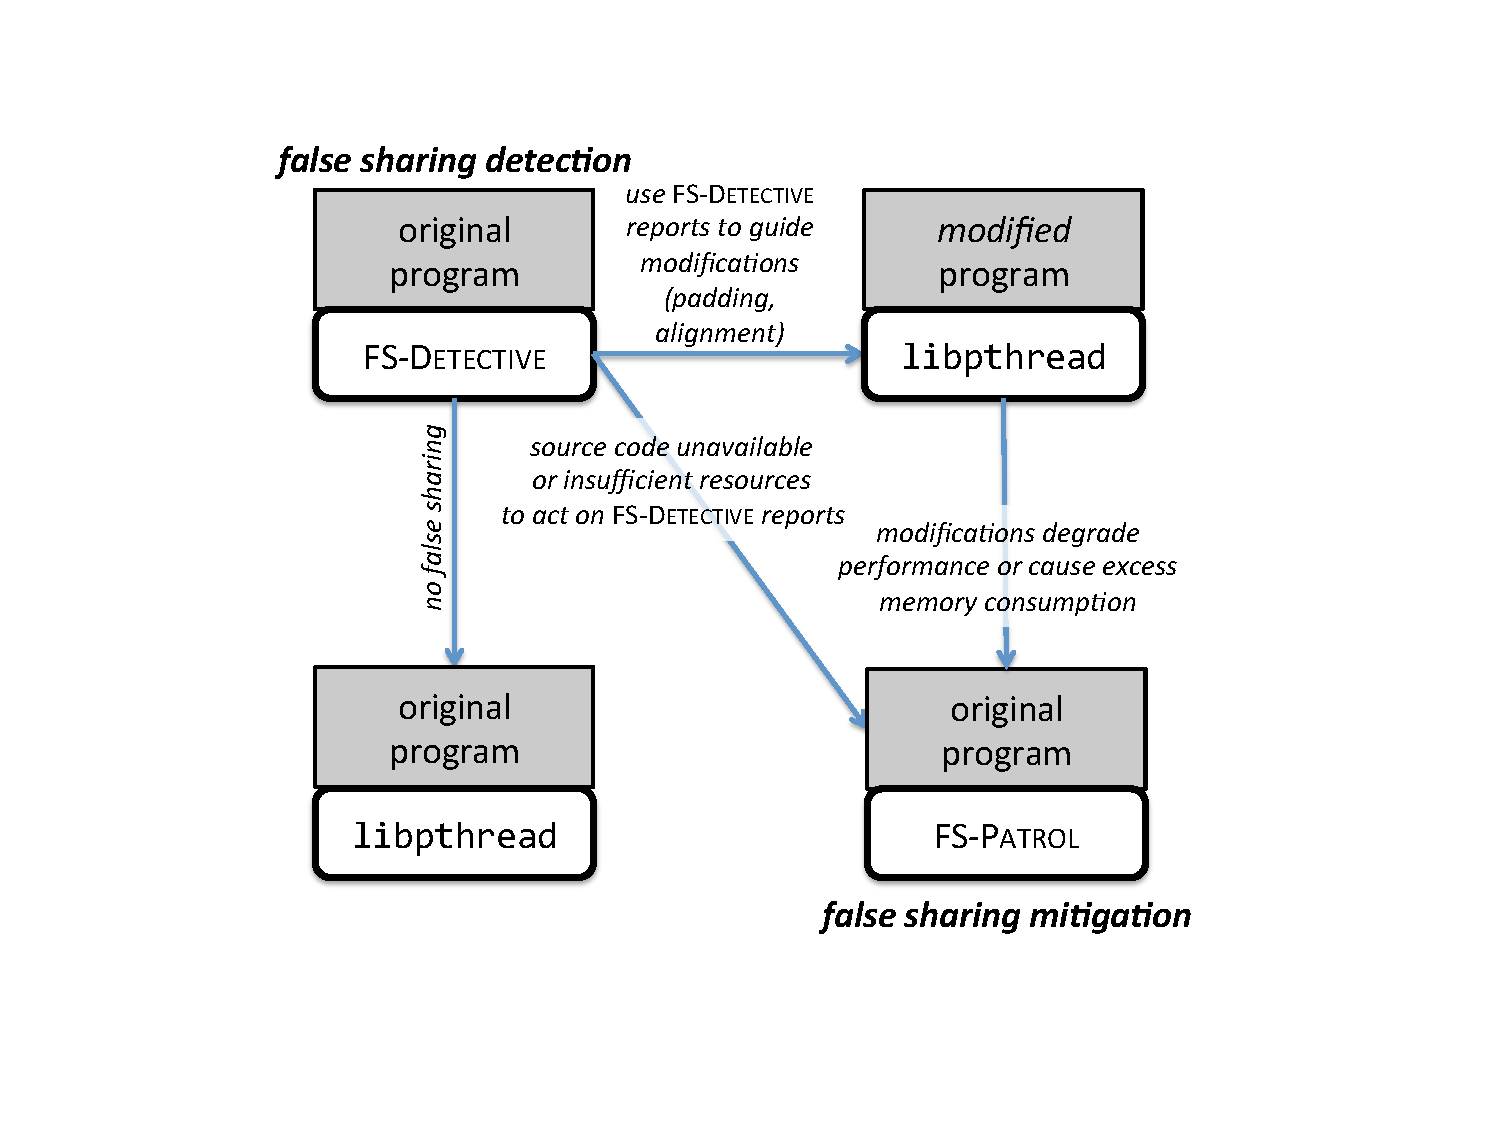
\includegraphics[width=3.2in]{figure/sheriff-usecase.pdf}
\caption{A workflow for using \sheriffdetect{} and \sheriffprotect{}. 
\label{fig:usecase}}
\end{figure}

We evaluate \sheriffdetect{} and \sheriffprotect{} over a range of
applications, including the Phoenix and PARSEC benchmark suites; the latter is designed to be representative of
next-generation shared-memory programs for
chip-multiprocessors~\cite{parsec}. We
show that \sheriffdetect{} can successfully guide programmers to the
exact sources of false sharing, and use its results to remove false
sharing in several applications. We also apply \sheriffprotect{} to
automatically mitigate false sharing in these applications; in one
case, an applicaton suffering from catastrophic false sharing runs
$9\times$ faster with \sheriffprotect{} than with the
standard \pthreads{} library.

\subsection*{Outline}

The remainder of this paper is organized as
follows. Section~\ref{sec:relatedwork} describes key related work.
Section~\ref{sec:simulation} describes \sheriff{}'s mechanisms and
algorithms in detail.
%%%% Tongping and presents \sheriff{}. 
Section~\ref{sec:falseshare} describes the \sheriffdetect{} tool and how it works to locate false sharing
problems.  
Section~\ref{sec:patrol} presents the \sheriffprotect{} runtime system.
%%% Section~\ref{discussion-perf} discusses some key performance optimizations and 
Section~\ref{sec:evaluation}
presents experimental results, including several
case studies of using
\sheriffdetect{} to detect and guide the correction of false sharing. Finally, Section~\ref{sec:conclusion} concludes.

% \end{comment}
